\documentclass{ximera}
\graphicspath{  %% When looking for images,
{./}            %% look here first,
{./pictures/}   %% then look for a pictures folder,
{../pictures/}  %% which may be a directory up.
{../../pictures/}  %% which may be a directory up.
{../../../pictures/}  %% which may be a directory up.
{../../../../pictures/}  %% which may be a directory up.
}

\usepackage{listings}
%\usepackage{circuitikz}
\usepackage{xcolor}
\usepackage{amsmath,amsthm}
\usepackage{subcaption}
\usepackage{graphicx}
\usepackage{tikz}
%\usepackage{tikz-3dplot}
\usepackage{amsfonts}
%\usepackage{mdframed} % For framing content
%\usepackage{tikz-cd}

  \renewcommand{\vector}[1]{\left\langle #1\right\rangle}
  \newcommand{\arrowvec}[1]{{\overset{\rightharpoonup}{#1}}}
  \newcommand{\ro}{\texttt{R}}%% row operation
  \newcommand{\dotp}{\bullet}%% dot product
  \renewcommand{\l}{\ell}
  \let\defaultAnswerFormat\answerFormatBoxed
  \usetikzlibrary{calc,bending}
  \tikzset{>=stealth}
  




%make a maroon color
\definecolor{maroon}{RGB}{128,0,0}
%make a dark blue color
\definecolor{darkblue}{RGB}{0,0,139}
%define the color fourier0 to be the maroon color
\definecolor{fourier0}{RGB}{128,0,0}
%define the color fourier1 to be the dark blue color
\definecolor{fourier1}{RGB}{0,0,139}
%define the color fourier 1t to be the light blue color
\definecolor{fourier1t}{RGB}{173,216,230}
%define the color fourier2 to be the dark green color
\definecolor{fourier2}{RGB}{0,100,0}
%define teh color fourier2t to be the light green color
\definecolor{fourier2t}{RGB}{144,238,144}
%define the color fourier3 to be the dark purple color
\definecolor{fourier3}{RGB}{128,0,128}
%define the color fourier3t to be the light purple color
\definecolor{fourier3t}{RGB}{221,160,221}
%define the color fourier0t to be the red color
\definecolor{fourier0t}{RGB}{255,0,0}
%define the color fourier4 to be the orange color
\definecolor{fourier4}{RGB}{255,165,0}
%define the color fourier4t to be the darker orange color
\definecolor{fourier4t}{RGB}{255,215,0}
%define the color fourier5 to be the yellow color
\definecolor{fourier5}{RGB}{255,255,0}
%define the color fourier5t to be the darker yellow color
\definecolor{fourier5t}{RGB}{255,255,100}
%define the color fourier6 to be the green color
\definecolor{fourier6}{RGB}{0,128,0}
%define the color fourier6t to be the darker green color
\definecolor{fourier6t}{RGB}{0,255,0}

%New commands for this doc for errors in copying
\newcommand{\eigenvar}{\lambda}
%\newcommand{\vect}[1]{\mathbf{#1}}
\renewcommand{\th}{^{\text{th}}}
\newcommand{\st}{^{\text{st}}}
\newcommand{\nd}{^{\text{nd}}}
\newcommand{\rd}{^{\text{rd}}}
\newcommand{\paren}[1]{\left(#1\right)}
\newcommand{\abs}[1]{\left|#1\right|}
\newcommand{\R}{\mathbb{R}}
\newcommand{\C}{\mathbb{C}}
\newcommand{\Hilb}{\mathbb{H}}
\newcommand{\qq}[1]{\text{#1}}
\newcommand{\Z}{\mathbb{Z}}
\newcommand{\N}{\mathbb{N}}
\newcommand{\q}[1]{\text{``#1''}}
%\newcommand{\mat}[1]{\begin{bmatrix}#1\end{bmatrix}}
\newcommand{\rref}{\text{reduced row echelon form}}
\newcommand{\ef}{\text{echelon form}}
\newcommand{\ohm}{\Omega}
\newcommand{\volt}{\text{V}}
\newcommand{\amp}{\text{A}}
\newcommand{\Seq}{\textbf{Seq}}
\newcommand{\Poly}{\textbf{P}}
\renewcommand{\quad}{\text{    }}
\newcommand{\roweq}{\simeq}
\newcommand{\rowop}{\simeq}
\newcommand{\rowswap}{\leftrightarrow}
\newcommand{\Mat}{\textbf{M}}
\newcommand{\Func}{\textbf{Func}}
\newcommand{\Hw}{\textbf{Hamming weight}}
\newcommand{\Hd}{\textbf{Hamming distance}}
\newcommand{\rank}{\text{rank}}
\newcommand{\longvect}[1]{\overrightarrow{#1}}
% Define the circled command
\newcommand{\circled}[1]{%
  \tikz[baseline=(char.base)]{
    \node[shape=circle,draw,inner sep=2pt,red,fill=red!20,text=black] (char) {#1};}%
}

% Define custom command \strikeh that just puts red text on the 2nd argument
\newcommand{\strikeh}[2]{\textcolor{red}{#2}}

% Define custom command \strikev that just puts red text on the 2nd argument
\newcommand{\strikev}[2]{\textcolor{red}{#2}}

%more new commands for this doc for errors in copying
\newcommand{\SI}{\text{SI}}
\newcommand{\kg}{\text{kg}}
\newcommand{\m}{\text{m}}
\newcommand{\s}{\text{s}}
\newcommand{\norm}[1]{\left\|#1\right\|}
\newcommand{\col}{\text{col}}
\newcommand{\sspan}{\text{span}}
\newcommand{\proj}{\text{proj}}
\newcommand{\set}[1]{\left\{#1\right\}}
\newcommand{\degC}{^\circ\text{C}}
\newcommand{\centroid}[1]{\overline{#1}}
\newcommand{\dotprod}{\boldsymbol{\cdot}}
%\newcommand{\coord}[1]{\begin{bmatrix}#1\end{bmatrix}}
\newcommand{\iprod}[1]{\langle #1 \rangle}
\newcommand{\adjoint}{^{*}}
\newcommand{\conjugate}[1]{\overline{#1}}
\newcommand{\eigenvarA}{\lambda}
\newcommand{\eigenvarB}{\mu}
\newcommand{\orth}{\perp}
\newcommand{\bigbracket}[1]{\left[#1\right]}
\newcommand{\textiff}{\text{ if and only if }}
\newcommand{\adj}{\text{adj}}
\newcommand{\ijth}{\emph{ij}^\text{th}}
\newcommand{\minor}[2]{M_{#2}}
\newcommand{\cofactor}{\text{C}}
\newcommand{\shift}{\textbf{shift}}
\newcommand{\startmat}[1]{
  \left[\begin{array}{#1}
}
\newcommand{\stopmat}{\end{array}\right]}
%a command to give a name to explorations and hints and theorems
\newcommand{\name}[1]{\begin{centering}\textbf{#1}\end{centering}}
\newcommand{\vect}[1]{\vec{#1}}
\newcommand{\dfn}[1]{\textbf{#1}}
\newcommand{\transpose}{\mathsf{T}}
\newcommand{\mtlb}[2][black]{\texttt{\textcolor{#1}{#2}}}
\newcommand{\RR}{\mathbb{R}} % Real numbers
\newcommand{\id}{\text{id}}
\newcommand{\coord}[1]{\langle#1\rangle}
\newcommand{\RREF}{\text{RREF}}
\newcommand{\Null}{\text{Null}}
\newcommand{\Nullity}{\text{Nullity}}
\newcommand{\Rank}{\text{Rank}}
\newcommand{\Col}{\text{Col}}
\newcommand{\Ef}{\text{EF}}
\newcommand{\boxprod}[3]{\abs{(#1\times#2)\cdot#3}}

\author{Zack Reed}
%borrowed from selinger linear algebra
\title{Learning Activity: }
\begin{document}
\begin{abstract}

    In this learning activity, you will be 
\end{abstract}
\maketitle


\section*{Homogeneous Coordinates in 2D: Linear Translation?}

    
We've given much attention to the use of linear transformations to alter the positions of vectors in space. While we can do many transformations like rotations, scales, shears, and more general transformations, one pressing constraint is that linear transformations must send $\vec{0}$ to $\vec{0}$. In other words, $\vec{0}$ is always in the kernel of a linear transformation. This poses a problem for a commonly desired transformation in animation - translation. This issue is examined below in 2D. You will then apply the same principle to enact 3D translation in your midterm projects.
    
Consider displaying the letter $A$. In reality, it is depicted on the screen, as in the figure below, by specifying the coordinates of the 11 corners and filling in the interior.
    
    \begin{center}
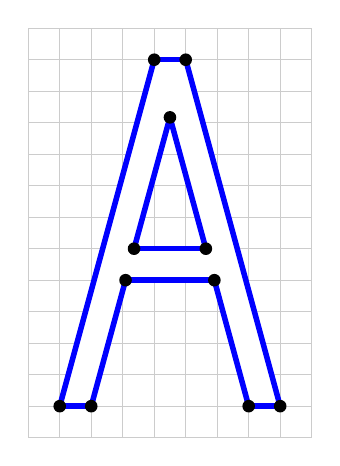
\begin{tikzpicture}[scale=0.4]
\draw[thin,gray!40] (0,0) grid (9,13);
    \filldraw[white, opacity=1](1,1)--(2.36,6)--(6.64,6)--(8,1)--(7,1)--(5.91,5)--(3.09,5)--(2,1)--cycle;
    \filldraw[white, opacity=1](2.36,6)--(4,12)--(5,12)--(6.64,6)--(5.64,6)--(4.5,10.17)--(3.36,6)--cycle;
    \draw[line width=2pt,blue](1,1)--(4,12);
    \draw[line width=2pt,blue](5,12)--(4,12);
    \draw[line width=2pt,blue](5,12)--(8,1);
    \draw[line width=2pt,blue](8,1)--(7,1);
    \draw[line width=2pt,blue](7,1)--(5.91,5);
    \draw[line width=2pt,blue](5.91,5)--(3.09,5);
    \draw[line width=2pt,blue](3.09,5)--(2,1);
    \draw[line width=2pt,blue](1,1)--(2,1);
    \draw[line width=2pt,blue](4.5,10.17)--(3.36,6);
    \draw[line width=2pt,blue](4.5,10.17)--(5.64,6);
    \draw[line width=2pt,blue](3.36,6)--(5.64,6);
    \fill[] (1,1) circle (0.2cm);
    \fill[] (4,12) circle (0.2cm);
    \fill[] (5,12) circle (0.2cm);
    \fill[] (8,1) circle (0.2cm);
    \fill[] (7,1) circle (0.2cm);
    \fill[] (5.91,5) circle (0.2cm);
    \fill[] (3.09,5) circle (0.2cm);
    \fill[] (2,1) circle (0.2cm);
    \fill[] (4.5,10.17) circle (0.2cm);
    \fill[] (3.36,6) circle (0.2cm);
    \fill[] (5.64,6) circle (0.2cm);
    \end{tikzpicture}
\end{center} 
    
    For simplicity, we will disregard the thickness of the letter,
    so we require only five coordinates as in the figure below.
    
    \begin{center}
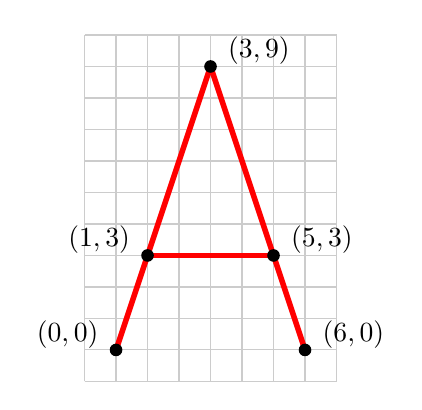
\begin{tikzpicture}[scale=0.4]
\draw[thin,gray!40] (-1,-1) grid (7,10);
    \draw[line width=2pt,red](0,0)--(3,9);
    \draw[line width=2pt,red](6,0)--(3,9);
    \draw[line width=2pt,red](5,3)--(1,3);
    \fill[] (0,0)node[above=2mm, left=1mm]{$(0,0)$} circle (0.2cm);
    \fill[] (6,0)node[above=2mm, right=1mm]{$(6,0)$} circle (0.2cm);
    \fill[] (5,3)node[above=2mm, right=1mm]{$(5,3)$} circle (0.2cm);
    \fill[] (1,3)node[above=2mm, left=1mm]{$(1,3)$} circle (0.2cm);
    \fill[] (3,9)node[above=2mm, right=1mm]{$(3,9)$} circle (0.2cm);
    \end{tikzpicture}
\end{center} 
    
This simplified letter can then be stored as a data matrix
    
$$D =\begin{bmatrix}
0 & 6 & 5 & 1 & 3\\
0 & 0 & 3 & 3 & 9
\end{bmatrix}$$
    
where the columns are the coordinates of the vertices. Then if we want to transform the letter by a $2 \times 2$ matrix $A$, we left-multiply this data matrix by $A$ (the effect is to multiply each column by $A$ and so transform each vertex).
    
For example, we can slant the letter to the right by multiplying by a horizontal shear matrix $A = \left[
\begin{array}{ll}
1 & 0.2\\
0 & 1\\
\end{array}
\right]$
    (See Formula \ref{form:shears}.) The result is the letter with data matrix
\begin{equation*}
A = \left[
\begin{array}{ll}
1 & 0.2\\
0 & 1
\end{array}
\right] \left[
\begin{array}{rrrrr}
0 & 6 & 5 & 1 & 3\\
0 & 0 & 3 & 3 & 9
\end{array}
\right] =
    \left[
\begin{array}{lllll}
0 & 6 & 5.6 & 1.6 & 4.8\\
0 & 0 & 3 & 3 & 9
\end{array}
\right]
\end{equation*}
which is shown in the figure below.
    
    \begin{center}
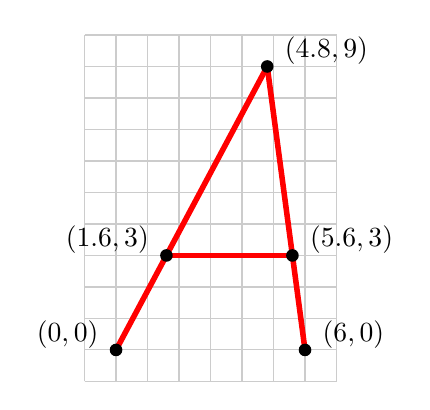
\begin{tikzpicture}[scale=0.4]
\draw[thin,gray!40] (-1,-1) grid (7,10);
    \draw[line width=2pt,red](0,0)--(4.8,9);
    \draw[line width=2pt,red](6,0)--(4.8,9);
    \draw[line width=2pt,red](5.6,3)--(1.6,3);
    \fill[] (0,0)node[above=2mm, left=1mm]{$(0,0)$} circle (0.2cm);
    \fill[] (6,0)node[above=2mm, right=1mm]{$(6,0)$} circle (0.2cm);
    \fill[] (5.6,3)node[above=2mm, right=1mm]{$(5.6,3)$} circle (0.2cm);
    \fill[] (1.6,3)node[above=2mm, left=1mm]{$(1.6,3)$} circle (0.2cm);
    \fill[] (4.8,9)node[above=2mm, right=1mm]{$(4.8,9)$} circle (0.2cm);
    \end{tikzpicture}
\end{center} 
    
    
    If we want to make this slanted matrix narrower, we can now apply a scaling matrix $B = \left[
\begin{array}{ll}
    0.8 & 0\\
    0 & 1
\end{array}
\right]$ that shrinks the $x$-coordinate by $0.8$. (See Formula \ref{form:horvertscaling}.) The result is the composite transformation
\begin{align*}
BAD &= \left[
\begin{array}{ll}
0.8 & 0\\
0 & 1
\end{array}
\right] \left[
\begin{array}{ll}
1 & 0.2\\
0 & 1
\end{array}
\right] \left[
\begin{array}{rrrrr}
0 & 6 & 5 & 1 & 3\\
0 & 0 & 3 & 3 & 9
\end{array}
\right] \\ &=
\left[
\begin{array}{lllll}
0 & 4.8 & 4.48 & 1.28 & 3.84\\
0 & 0 & 3 & 3 & 9
\end{array}
\right]
\end{align*}
which is drawn in the figure below.
    
    \begin{center}
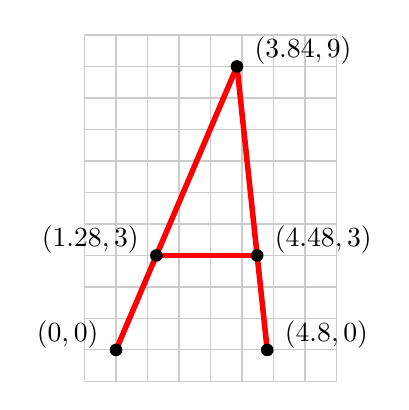
\begin{tikzpicture}[scale=0.4]
\draw[thin,gray!40] (-1,-1) grid (7,10);
    \draw[line width=2pt,red](0,0)--(3.84,9);
    \draw[line width=2pt,red](4.8,0)--(3.84,9);
    \draw[line width=2pt,red](4.48,3)--(1.28,3);
    \fill[] (0,0)node[above=2mm, left=1mm]{$(0,0)$} circle (0.2cm);
    \fill[] (4.8,0)node[above=2mm, right=1mm]{$(4.8,0)$} circle (0.2cm);
    \fill[] (4.48,3)node[above=2mm, right=1mm]{$(4.48,3)$} circle (0.2cm);
    \fill[] (1.28,3)node[above=2mm, left=1mm]{$(1.28,3)$} circle (0.2cm);
    \fill[] (3.84,9)node[above=2mm, right=1mm]{$(3.84,9)$} circle (0.2cm);
    \end{tikzpicture}
\end{center} 
    
On the other hand, we can rotate the letter about the origin through $\frac{\pi}{6}$ (or $30^\circ$) by multiplying by the rotation matrix  $$R_{\frac{\pi}{2}} = \left[
\def\arraystretch{1.5}\begin{array}{rr}
\cos(\frac{\pi}{6}) & -\sin(\frac{\pi}{6})\\
\sin(\frac{\pi}{6}) & \cos(\frac{\pi}{6})
\end{array}
\right] = \left[
\begin{array}{ll}
0.866 & -0.5\\
0.5 & 0.866
\end{array}
\right]$$
(See Formula \ref{form:rotation}.)  This gives
\begin{align*}
R_{\frac{\pi}{2}} &= \left[
\begin{array}{ll}
0.866 & -0.5\\
0.5 & 0.866
\end{array}
\right] \left[
\begin{array}{rrrrr}
0 & 6 & 5 & 1 & 3\\
0 & 0 & 3 & 3 & 9
\end{array}
\right] \\ &=
\left[
\begin{array}{lllrr}
0 & 5.196 & 2.83 & -0.634 & -1.902\\
0 & 3 & 5.098 & 3.098 & 9.294
\end{array}
\right]
\end{align*}
and is plotted in the figure below.
    
    \begin{center}
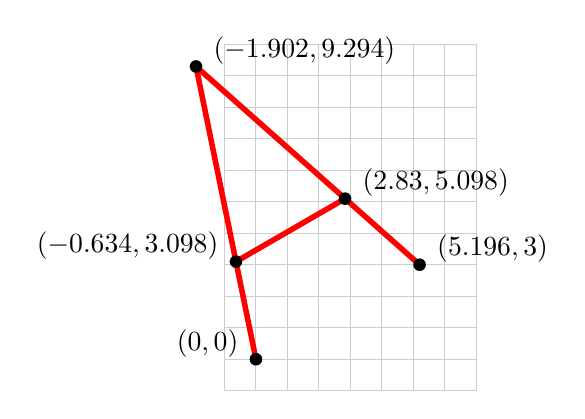
\begin{tikzpicture}[scale=0.4]
\draw[thin,gray!40] (-1,-1) grid (7,10);
    \draw[line width=2pt,red](0,0)--(-1.902,9.294);
    \draw[line width=2pt,red](-0.634,3.098)--(2.83,5.098);
    \draw[line width=2pt,red](5.196,3)--(-1.902,9.294);
    \fill[] (0,0)node[above=2mm, left=1mm]{$(0,0)$} circle (0.2cm);
    \fill[] (2.83,5.098)node[above=2mm, right=1mm]{$(2.83,5.098)$} circle (0.2cm);
    \fill[] (5.196,3)node[above=2mm, right=1mm]{$(5.196,3)$} circle (0.2cm);
    \fill[] (-0.634,3.098)node[above=2mm, left=1mm]{$(-0.634,3.098)$} circle (0.2cm);
    \fill[] (-1.902,9.294)node[above=2mm, right=1mm]{$(-1.902,9.294)$} circle (0.2cm);
    \end{tikzpicture}
\end{center} 
    
This poses a problem: How do we rotate
about a point other than the origin? It turns out that we can do this when
we have solved another more basic problem. It is clearly important to be
    able to translate a screen image by a fixed vector $\vec{w}$, that is apply the transformation $T_{w} : \RR^2 \to \RR^2$ given by $T_{w}(\vec{v}) = \vec{v} + \vec{w}$ for all $\vec{v}$ in $\RR^2$. The problem is that these translations are not matrix transformations $\RR^2 \to \RR^2$ because they do not carry $\vec{0}$ to $\vec{0}$ (unless $\vec{w} = \vec{0}$). (See Practice Problem \ref{prob:translation_does_not_work}.) However, there is a clever way around this.
    
The idea is to represent a point $\vec{v} = \left[
\begin{array}{r}
x\\
y
\end{array}
\right]$
    as a $3 \times 1$ column $\left[
    \begin{array}{r}
    x\\
    y\\
    1
    \end{array}
    \right]$, called the \dfn{homogeneous coordinates}\index{homogeneous coordinates} of $\vec{v}$. Then translation by $\vec{w} = \left[
    \begin{array}{r}
    p\\
    q
    \end{array}
    \right]$ can be achieved by multiplying by a $3 \times 3$ matrix:
\begin{equation*}
\left[
\begin{array}{rrr}
1 & 0 & p\\
0 & 1 & q\\
0 & 0 & 1
\end{array}
\right] \left[
\begin{array}{r}
x\\
y\\
1
\end{array}
\right]
=
\left[
\begin{array}{c}
x + p\\
y + q\\
1
\end{array}
\right]
=
\left[
\begin{array}{c}
T_{\vec{w}}(\vec{v})\\
1
\end{array}
\right]
\end{equation*}
Thus, by using homogeneous coordinates we can implement the translation $T_{w}$ in the top two coordinates. At the same time, matrix transformations we performed earlier can still be accomplished using homogeneous coordinates.  For instance, the matrix transformation induced by $A = \left[
\begin{array}{rr}
a & b\\
c & d
\end{array}
\right]$ is given by a $3 \times 3$ matrix:
\begin{equation*}
\left[
\begin{array}{rrr}
a & b & 0\\
c & d & 0\\
0 & 0 & 1
\end{array}
\right] \left[
\begin{array}{r}
x\\
y\\
1
\end{array}
\right]
=
\left[
\begin{array}{c}
ax + by\\
cx + dy\\
1
\end{array}
\right]
=
\left[
\begin{array}{c}
A\vec{v}\\
1
\end{array}
\right]
\end{equation*}
So everything can be accomplished at the expense of using $3 \times 3$ matrices and homogeneous coordinates.
    
It is interesting to examine the geometric implications of homogeneous coordinates.  All points of the form $\begin{bmatrix}x\\y\end{bmatrix}$, originally located in the $xy$-plane in $\RR^2$, now have the form $\begin{bmatrix}x\\y\\1\end{bmatrix}$ and are located in a horizontal plane $z=1$ in $\RR^3$.  What we perceive as a translation in the horizontal plane $z=1$, is actually a shear in $\RR^3$.  This is similar to how horizontal shears in $\RR^2$ affect points along the line $y=1$: all such points move a fixed distance to the left or to the right.
    
    
\begin{example}\label{exa:013322}
Rotate the letter $A$ through $\frac{\pi}{6}$ about the point $\left[
\begin{array}{c}
4\\
5
\end{array}
\right]$.
    
\begin{center}
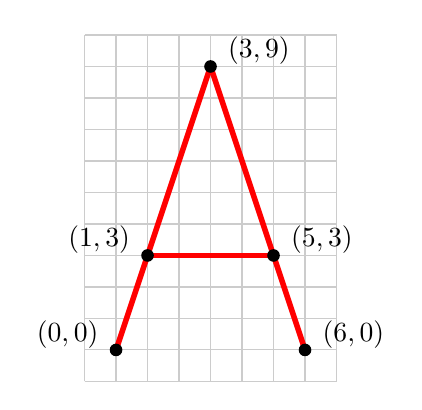
\begin{tikzpicture}[scale=0.4]
\draw[thin,gray!40] (-1,-1) grid (7,10);
    \draw[line width=2pt,red](0,0)--(3,9);
    \draw[line width=2pt,red](6,0)--(3,9);
    \draw[line width=2pt,red](5,3)--(1,3);
    \fill[] (0,0)node[above=2mm, left=1mm]{$(0,0)$} circle (0.2cm);
    \fill[] (6,0)node[above=2mm, right=1mm]{$(6,0)$} circle (0.2cm);
    \fill[] (5,3)node[above=2mm, right=1mm]{$(5,3)$} circle (0.2cm);
    \fill[] (1,3)node[above=2mm, left=1mm]{$(1,3)$} circle (0.2cm);
    \fill[] (3,9)node[above=2mm, right=1mm]{$(3,9)$} circle (0.2cm);
    \end{tikzpicture}
\end{center}
    
\begin{explanation}
Using homogenous coordinates for the vertices of the letter results in a data matrix with three rows:
\begin{equation*}
K_{d} =  \left[
\begin{array}{rrrrr}
0 & 6 & 5 & 1 & 3\\
0 & 0 & 3 & 3 & 9 \\
1 & 1 & 1 & 1 & 1
\end{array}
\right]
\end{equation*}
    
%\begin{wrapfigure}[6]{l}{5cm}
%\vspace*{-5em}
%\centering
%\input{4-vector-geometry/figures/5-an-application-to-computer-graphics/figure4.5.6}
%\caption{\label{fig:013335}}
%\end{wrapfigure}
    
    
If we write $\vec{w} = \left[
\begin{array}{c}
4\\
5
\end{array}
\right]$, the idea is to use a composite of transformations: First translate the letter by $-\vec{w}$ so that the point $\vec{w}$ moves to the origin, then rotate this translated letter, and then translate it by $\vec{w}$ back to its original position. The following GeoGebra interactive illustrates this sequence.
    
\pdfOnly{
Access GeoGebra interactives through the online version of this text at
    
\href{https://ximera.osu.edu/oerlinalg}{https://ximera.osu.edu/oerlinalg}.
}
    
\begin{onlineOnly}
\begin{center}
\geogebra{yd5agbdg}{950}{650}
\end{center}
\end{onlineOnly}
    
The matrix arithmetic is as follows (remember the order of composition!):
\begin{align*}
& \left[
\begin{array}{rrr}
1 & 0 & 4\\
0 & 1 & 5\\
0 & 0 & 1
\end{array}
\right]
\left[
\begin{array}{lrr}
0.866 & -0.5 & 0\\
0.5 & 0.866 & 0\\
0 & 0 & 1
\end{array}
\right]
\left[
\begin{array}{rrr}
1 & 0 & -4\\
0 & 1 & -5\\
0 & 0 & 1
\end{array}
\right]
\left[
\begin{array}{rrrrr}
0 & 6 & 5 & 1 & 3\\
0 & 0 & 3 & 3 & 9 \\
1 & 1 & 1 & 1 & 1
\end{array}
\right] \\
&= \left[
\begin{array}{lllll}
3.036 & 8.232 & 5.866 & 2.402 & 1.134\\
-1.33 & 1.67 & 3.768 & 1.768 & 7.964 \\
1 & 1 & 1 & 1 & 1
\end{array}
\right]
\end{align*}
    
\end{explanation}
\end{example}
    
This discussion merely touches the
surface of computer graphics, and the reader is referred to specialized
books on the subject. Realistic graphic rendering requires an enormous
number of matrix calculations. In fact, matrix multiplication algorithms
    are now embedded in microchip circuits, and can perform over 100
million matrix multiplications per second. This is particularly
important in the field of three-dimensional graphics where the
homogeneous coordinates have four components and $4 \times 4$ matrices are
required.
    
    
\section*{Practice Problems}
    
\begin{problem}\label{prob:app0040_1}
Consider the letter $A$ below.
\begin{center}
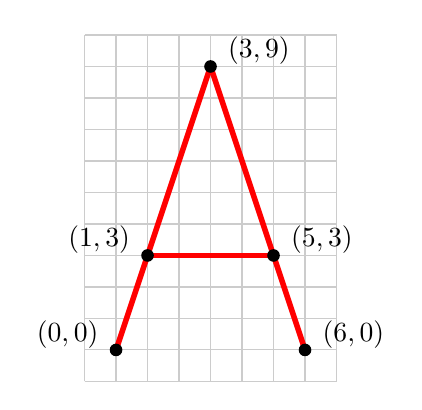
\begin{tikzpicture}[scale=0.4]
\draw[thin,gray!40] (-1,-1) grid (7,10);
    \draw[line width=2pt,red](0,0)--(3,9);
    \draw[line width=2pt,red](6,0)--(3,9);
    \draw[line width=2pt,red](5,3)--(1,3);
    \fill[] (0,0)node[above=2mm, left=1mm]{$(0,0)$} circle (0.2cm);
    \fill[] (6,0)node[above=2mm, right=1mm]{$(6,0)$} circle (0.2cm);
    \fill[] (5,3)node[above=2mm, right=1mm]{$(5,3)$} circle (0.2cm);
    \fill[] (1,3)node[above=2mm, left=1mm]{$(1,3)$} circle (0.2cm);
    \fill[] (3,9)node[above=2mm, right=1mm]{$(3,9)$} circle (0.2cm);
    \end{tikzpicture}
\end{center} 
    
Find the data matrix for the letter obtained by:
    
    
\begin{enumerate}
\item Rotating the letter through $\frac{\pi}{4}$ about the origin.
    
\item Rotating the letter through $\frac{\pi}{4}$
    about the point $\left[
    \begin{array}{c}
    1\\
    2
    \end{array}
    \right]$.
    
Click the arrow to see the answer.

${\frac{1}{2}\left[
\begin{array}{ccccc}
\sqrt{2} + 2 & 7\sqrt{2} + 2 & 3\sqrt{2} + 2 & -\sqrt{2} + 2 & -5\sqrt{2} + 2\\
-3\sqrt{2} + 4 & 3\sqrt{2} + 4 & 5\sqrt{2} + 4 & \sqrt{2} + 4 & 9\sqrt{2} + 4 \\
2 & 2 & 2 & 2 & 2
\end{array}
\right]}$

\end{enumerate}
\end{problem}
    
% \begin{problem}\label{prob:app0040_2}
% Find the matrix for turning the letter $A$ in Figure~\ref{fig:013290} upside-down in place.
% \end{problem}
    
\begin{problem}\label{prob:app0040_3}
Find the $3 \times 3$ matrix for reflecting in the line $y = mx + b$. Use $\left[
\begin{array}{c}
1\\
m
\end{array}
\right]$ as direction vector for the line.
\end{problem}
    
\begin{problem}\label{prob:app0040_4}
Find the $3 \times 3$ matrix for rotating through the angle $\theta$ about the point $P(a, b)$.
\end{problem}
    
\begin{problem}\label{prob:app0040_5}
Find the reflection of the point $P$ in the line $y = 1 + 2x$ in $\RR^2$ if:
    
    
\begin{enumerate}
\item $P = P(1, 1)$
    
\item $P = P(1, 4)$
    
Click the arrow to see the answer.

$P(\frac{9}{5}, \frac{18}{5})$

    
\item What about $P = P(1, 3)$? Explain.
\begin{hint}
    See Example~\ref{exa:013322}.
\end{hint}
\end{enumerate}
\end{problem}
    
\end{document}